\documentclass[tikz,border=10pt]{standalone}
\usepackage{tikz}
\usetikzlibrary{arrows.meta,positioning,shapes}
\usepackage{amsmath} % <<<<<<  AÑADIDO


\begin{document}
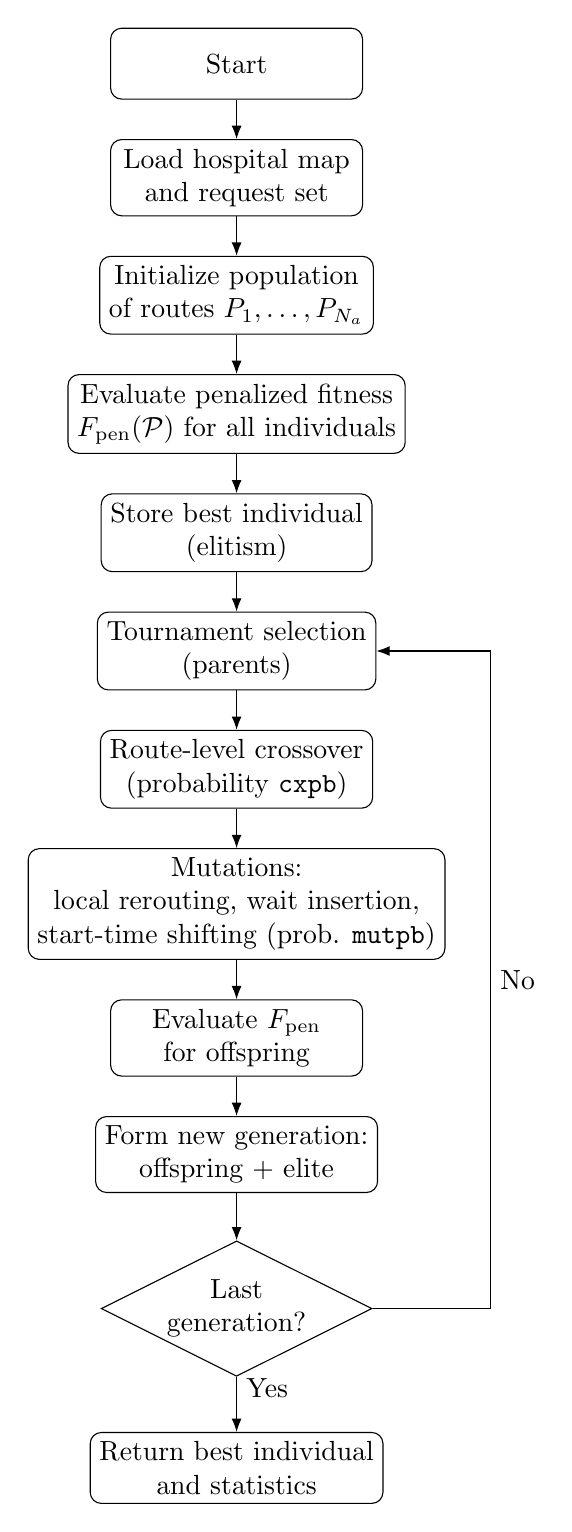
\begin{tikzpicture}[
  node distance=0.5cm,
  >=Latex,
  block/.style={rectangle, draw, rounded corners, align=center, minimum width=3.2cm, minimum height=0.9cm},
  decision/.style={diamond, draw, aspect=2, align=center, inner sep=1pt},
  line/.style={draw, -{Latex}}
]

\node[block] (start) {Start};
\node[block, below=of start] (env) {Load hospital map\\and request set};
\node[block, below=of env] (init) {Initialize population\\of routes $P_1,\dots,P_{N_a}$};
\node[block, below=of init] (eval) {Evaluate penalized fitness\\$F_{\text{pen}}(\mathcal{P})$ for all individuals};
\node[block, below=of eval] (elite) {Store best individual\\(elitism)};
\node[block, below=of elite] (select) {Tournament selection\\(parents)};
\node[block, below=of select] (crossover) {Route-level crossover\\(probability \texttt{cxpb})};
\node[block, below=of crossover] (mutation) {Mutations:\\local rerouting, wait insertion,\\start-time shifting (prob. \texttt{mutpb})};
\node[block, below=of mutation] (eval2) {Evaluate $F_{\text{pen}}$\\for offspring};
\node[block, below=of eval2] (replace) {Form new generation:\\offspring $+$ elite};
\node[decision, below=of replace, yshift=-0.1cm] (stop) {Last\\generation?};
\node[block, below=of stop, yshift=-0.2cm] (end) {Return best individual\\and statistics};

\path[line] (start) -- (env);
\path[line] (env) -- (init);
\path[line] (init) -- (eval);
\path[line] (eval) -- (elite);
\path[line] (elite) -- (select);
\path[line] (select) -- (crossover);
\path[line] (crossover) -- (mutation);
\path[line] (mutation) -- (eval2);
\path[line] (eval2) -- (replace);
\path[line] (replace) -- (stop);

\path[line] (stop.east) -- ++(1.5,0) |- (select.east) node[pos=0.25, right]{No};
\path[line] (stop.south) -- (end.north) node[pos=0.2, right]{Yes};

\end{tikzpicture}
\end{document}
